% Generated by code/needham.py -- do not edit by hand.
\definecolor{qocA}{rgb}{0.00,0.45,0.70}
\definecolor{qocB}{rgb}{0.90,0.60,0.00}
\definecolor{qocC}{rgb}{0.00,0.62,0.45}
\definecolor{qocD}{rgb}{0.80,0.40,0.00}
\definecolor{qocE}{rgb}{0.80,0.60,0.70}
\definecolor{qocF}{rgb}{0.35,0.70,0.90}
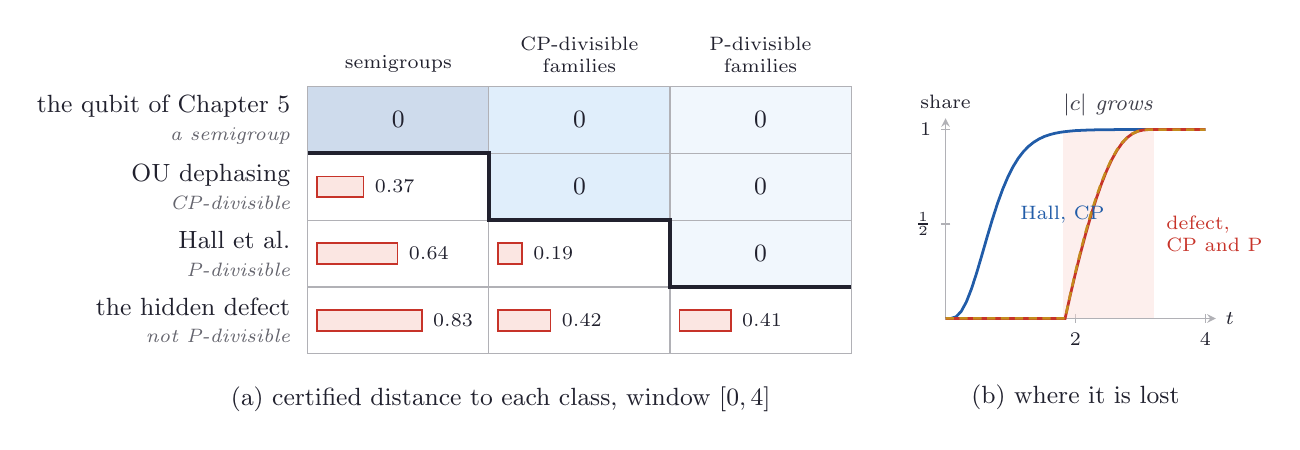
\begin{tikzpicture}[ink/.style={line width=0.9pt, ndInk}, faint/.style={line width=0.4pt, ndInk!35}, dashedink/.style={line width=0.5pt, ndInk!55, dash pattern=on 2.5pt off 2pt}, vec/.style={->, >=stealth, line width=1.2pt}, note/.style={font=\footnotesize\itshape, text=ndInk!85, align=center}, pointer/.style={->, >=stealth, line width=0.4pt, ndInk!60, shorten >=2pt, shorten <=1pt}, dot/.style={circle, fill=ndInk, inner sep=0pt, minimum size=3.4pt}, wash/.style={fill=ndSky, fill opacity=0.55}, every node/.style={text=ndInk}]
\definecolor{ndInk}{rgb}{0.13,0.13,0.18}
\definecolor{ndPaper}{rgb}{0.99,0.96,0.88}
\definecolor{ndSky}{rgb}{0.84,0.91,0.98}
\definecolor{ndRose}{rgb}{0.98,0.86,0.84}
\definecolor{ndBlue}{rgb}{0.13,0.36,0.66}
\definecolor{ndRed}{rgb}{0.78,0.20,0.16}
\definecolor{ndGold}{rgb}{0.88,0.62,0.10}
\definecolor{ndGreen}{rgb}{0.18,0.52,0.30}
\node[font=\scriptsize, align=center, anchor=south] at (4.050,4.150) {semigroups};
\node[font=\scriptsize, align=center, anchor=south] at (6.350,4.150) {CP-divisible\\ families};
\node[font=\scriptsize, align=center, anchor=south] at (8.650,4.150) {P-divisible\\ families};
\node[font=\small, anchor=east, align=right] at (2.800,3.675) {the qubit of Chapter 5\\[-1pt]{\scriptsize\itshape\color{ndInk!70} a semigroup}};
\fill[ndBlue!22] (2.900,3.250) rectangle (5.200,4.100);
\node[font=\small] at (4.050,3.675) {$0$};
\fill[ndSky!75] (5.200,3.250) rectangle (7.500,4.100);
\node[font=\small] at (6.350,3.675) {$0$};
\fill[ndSky!35] (7.500,3.250) rectangle (9.800,4.100);
\node[font=\small] at (8.650,3.675) {$0$};
\node[font=\small, anchor=east, align=right] at (2.800,2.825) {OU dephasing\\[-1pt]{\scriptsize\itshape\color{ndInk!70} CP-divisible}};
\fill[ndRose!70] (3.020,2.695) rectangle (3.607,2.955);
\draw[ndRed, line width=0.6pt] (3.020,2.695) rectangle (3.607,2.955);
\node[font=\scriptsize, anchor=west] at (3.627,2.825) {$0.37$};
\fill[ndSky!75] (5.200,2.400) rectangle (7.500,3.250);
\node[font=\small] at (6.350,2.825) {$0$};
\fill[ndSky!35] (7.500,2.400) rectangle (9.800,3.250);
\node[font=\small] at (8.650,2.825) {$0$};
\node[font=\small, anchor=east, align=right] at (2.800,1.975) {Hall et al.\\[-1pt]{\scriptsize\itshape\color{ndInk!70} P-divisible}};
\fill[ndRose!70] (3.020,1.845) rectangle (4.041,2.105);
\draw[ndRed, line width=0.6pt] (3.020,1.845) rectangle (4.041,2.105);
\node[font=\scriptsize, anchor=west] at (4.061,1.975) {$0.64$};
\fill[ndRose!70] (5.320,1.845) rectangle (5.621,2.105);
\draw[ndRed, line width=0.6pt] (5.320,1.845) rectangle (5.621,2.105);
\node[font=\scriptsize, anchor=west] at (5.641,1.975) {$0.19$};
\fill[ndSky!35] (7.500,1.550) rectangle (9.800,2.400);
\node[font=\small] at (8.650,1.975) {$0$};
\node[font=\small, anchor=east, align=right] at (2.800,1.125) {the hidden defect\\[-1pt]{\scriptsize\itshape\color{ndInk!70} not P-divisible}};
\fill[ndRose!70] (3.020,0.995) rectangle (4.349,1.255);
\draw[ndRed, line width=0.6pt] (3.020,0.995) rectangle (4.349,1.255);
\node[font=\scriptsize, anchor=west] at (4.369,1.125) {$0.83$};
\fill[ndRose!70] (5.320,0.995) rectangle (5.984,1.255);
\draw[ndRed, line width=0.6pt] (5.320,0.995) rectangle (5.984,1.255);
\node[font=\scriptsize, anchor=west] at (6.004,1.125) {$0.42$};
\fill[ndRose!70] (7.620,0.995) rectangle (8.273,1.255);
\draw[ndRed, line width=0.6pt] (7.620,0.995) rectangle (8.273,1.255);
\node[font=\scriptsize, anchor=west] at (8.293,1.125) {$0.41$};
\draw[faint] (2.900,4.100) -- (9.800,4.100);
\draw[faint] (2.900,3.250) -- (9.800,3.250);
\draw[faint] (2.900,2.400) -- (9.800,2.400);
\draw[faint] (2.900,1.550) -- (9.800,1.550);
\draw[faint] (2.900,0.700) -- (9.800,0.700);
\draw[faint] (2.900,4.100) -- (2.900,0.700);
\draw[faint] (5.200,4.100) -- (5.200,0.700);
\draw[faint] (7.500,4.100) -- (7.500,0.700);
\draw[faint] (9.800,4.100) -- (9.800,0.700);
\draw[line width=1.3pt, ndInk] (2.900,3.250) -- (5.200,3.250) -- (5.200,2.400) -- (7.500,2.400) -- (7.500,1.550) -- (9.800,1.550);
\node[font=\small, anchor=north] at (5.350,0.400) {(a) certified distance to each class, window $[0,4]$};
\draw[faint, ->, >=stealth] (11.000,1.150) -- (14.432,1.150) node[right, text=ndInk] {{\scriptsize $t$}};
\draw[faint, ->, >=stealth] (11.000,1.150) -- (11.000,3.694) node[above, text=ndInk] {{\scriptsize share}};
\draw[faint] (12.650,1.210) -- (12.650,1.090) node[below, font=\scriptsize, text=ndInk] {$2$};
\draw[faint] (14.300,1.210) -- (14.300,1.090) node[below, font=\scriptsize, text=ndInk] {$4$};
\draw[faint] (11.060,2.350) -- (10.940,2.350) node[left, font=\scriptsize, text=ndInk] {$\frac12$};
\draw[faint] (11.060,3.550) -- (10.940,3.550) node[left, font=\scriptsize, text=ndInk] {$1$};
\fill[ndRose, fill opacity=0.45] (12.493,1.150) rectangle (13.648,3.550);
\draw[line width=1.0pt, ndBlue] (11.000,1.150) -- (11.066,1.150) -- (11.132,1.171) -- (11.198,1.239) -- (11.264,1.360) -- (11.330,1.529) -- (11.396,1.733) -- (11.462,1.957) -- (11.528,2.186) -- (11.594,2.407) -- (11.660,2.612) -- (11.726,2.793) -- (11.792,2.949) -- (11.858,3.079) -- (11.924,3.186) -- (11.990,3.271) -- (12.056,3.338) -- (12.122,3.390) -- (12.188,3.430) -- (12.254,3.461) -- (12.320,3.484) -- (12.386,3.501) -- (12.452,3.514) -- (12.518,3.523) -- (12.584,3.530) -- (12.650,3.536) -- (12.716,3.539) -- (12.782,3.542) -- (12.848,3.544) -- (12.914,3.546) -- (12.980,3.547) -- (13.046,3.548) -- (13.112,3.548) -- (13.178,3.549) -- (13.244,3.549) -- (13.310,3.549) -- (13.376,3.550) -- (13.442,3.550) -- (13.508,3.550) -- (13.574,3.550) -- (13.640,3.550) -- (13.706,3.550) -- (13.772,3.550) -- (13.838,3.550) -- (13.904,3.550) -- (13.970,3.550) -- (14.036,3.550) -- (14.102,3.550) -- (14.168,3.550) -- (14.234,3.550) -- (14.300,3.550);
\draw[line width=1.0pt, ndRed] (11.000,1.150) -- (11.066,1.150) -- (11.132,1.150) -- (11.198,1.150) -- (11.264,1.150) -- (11.330,1.150) -- (11.396,1.150) -- (11.462,1.150) -- (11.528,1.150) -- (11.594,1.150) -- (11.660,1.150) -- (11.726,1.150) -- (11.792,1.150) -- (11.858,1.150) -- (11.924,1.150) -- (11.990,1.150) -- (12.056,1.150) -- (12.122,1.150) -- (12.188,1.150) -- (12.254,1.150) -- (12.320,1.150) -- (12.386,1.150) -- (12.452,1.150) -- (12.518,1.150) -- (12.584,1.447) -- (12.650,1.726) -- (12.716,1.988) -- (12.782,2.234) -- (12.848,2.463) -- (12.914,2.672) -- (12.980,2.861) -- (13.046,3.027) -- (13.112,3.170) -- (13.178,3.287) -- (13.244,3.380) -- (13.310,3.450) -- (13.376,3.498) -- (13.442,3.528) -- (13.508,3.543) -- (13.574,3.549) -- (13.640,3.550) -- (13.706,3.550) -- (13.772,3.550) -- (13.838,3.550) -- (13.904,3.550) -- (13.970,3.550) -- (14.036,3.550) -- (14.102,3.550) -- (14.168,3.550) -- (14.234,3.550) -- (14.300,3.550);
\draw[line width=0.9pt, ndGold!85!ndInk, dash pattern=on 3pt off 2pt] (11.000,1.150) -- (11.066,1.150) -- (11.132,1.150) -- (11.198,1.150) -- (11.264,1.150) -- (11.330,1.150) -- (11.396,1.150) -- (11.462,1.150) -- (11.528,1.150) -- (11.594,1.150) -- (11.660,1.150) -- (11.726,1.150) -- (11.792,1.150) -- (11.858,1.150) -- (11.924,1.150) -- (11.990,1.150) -- (12.056,1.150) -- (12.122,1.150) -- (12.188,1.150) -- (12.254,1.150) -- (12.320,1.150) -- (12.386,1.150) -- (12.452,1.150) -- (12.518,1.150) -- (12.584,1.457) -- (12.650,1.744) -- (12.716,2.012) -- (12.782,2.260) -- (12.848,2.488) -- (12.914,2.695) -- (12.980,2.880) -- (13.046,3.043) -- (13.112,3.181) -- (13.178,3.295) -- (13.244,3.385) -- (13.310,3.453) -- (13.376,3.499) -- (13.442,3.528) -- (13.508,3.544) -- (13.574,3.549) -- (13.640,3.550) -- (13.706,3.550) -- (13.772,3.550) -- (13.838,3.550) -- (13.904,3.550) -- (13.970,3.550) -- (14.036,3.550) -- (14.102,3.550) -- (14.168,3.550) -- (14.234,3.550) -- (14.300,3.550);
\node[font=\scriptsize, anchor=west, text=ndBlue] at (11.825,2.470) {Hall, CP};
\node[font=\scriptsize, anchor=west, text=ndRed, align=left] at (13.681,2.230) {defect,\\ CP and P};
\node[note, anchor=south] at (13.062,3.598) {$|c|$ grows};
\node[font=\small, anchor=north] at (12.650,0.430) {(b) where it is lost};
\end{tikzpicture}
